\clearpage
\subsection{Full-curve Monte Carlo assessment}

The full-curve evaluation reconstructs the same 3,000 data sets and estimator settings from the stored seeds, as recorded in \path{CURVE_SIMULATION_PLAN_20260916.md}. Each fit supplies five effects on $\{-0.8,-0.75,\ldots,0.8\}$. With generating correlation $r$, the moments $v_M=1$, $\omega_t=-0.8+t+r$ and $v_t=\omega_t^2+1-r^2$ give the main article's population curve. The total effect is 0.78 throughout; direct effects follow by subtraction.

For assumed $\rho$, bias, RMSE and coverage target the population sensitivity functional; \texttt{CausalBias} and \texttt{CausalInclusion} target the generating causal effect. Paired ratios use common valid replication identifiers. Monte Carlo calculations preserve within-curve dependence and use the valid-fit or all-attempt denominators defined in Section~\ref{sec:paired-audit}.

For a common assumed correlation, write $h=\rho/\sqrt{1-\rho^2}$. Each fitted effect has the exact form
\[
\widehat g(\rho)=\widehat A+h\widehat B,\qquad
\widehat\Var\{\widehat g(\rho)\}
=\widehat V_A+2h\widehat C_{AB}+h^2\widehat V_B.
\]
Here $A=g(\theta;0)$ and $B=g(\theta;1/\sqrt2)-g(\theta;0)$, with gradients obtained from the previously displayed effect map. The covariance terms follow jointly from the complete nuisance sandwich. The project repository stores these five coefficients for every effect and attempted fit, allowing all grid values and intervals to be reconstructed exactly for any plotting grid without refitting, smoothing or interpolating confidence limits. Unsuccessful fits retain missing coefficients and a diagnostic message.

The main figure's central 90\% empirical ranges describe the sampling distribution of the effect estimates across valid fits. Figure~\ref{fig:curve-coverage} separately evaluates each fit's nominal 95\% pointwise interval, and Figure~\ref{fig:curve-ratios} compares RMSE on paired valid data sets. Reading the RMSE ratios together with pointwise coverage is particularly informative where the estimated curve is near zero. Table~\ref{tab:curve-thresholds} adds a distinct evaluation of the estimated point-effect zero boundary.

\begin{figure}[p]
\centering
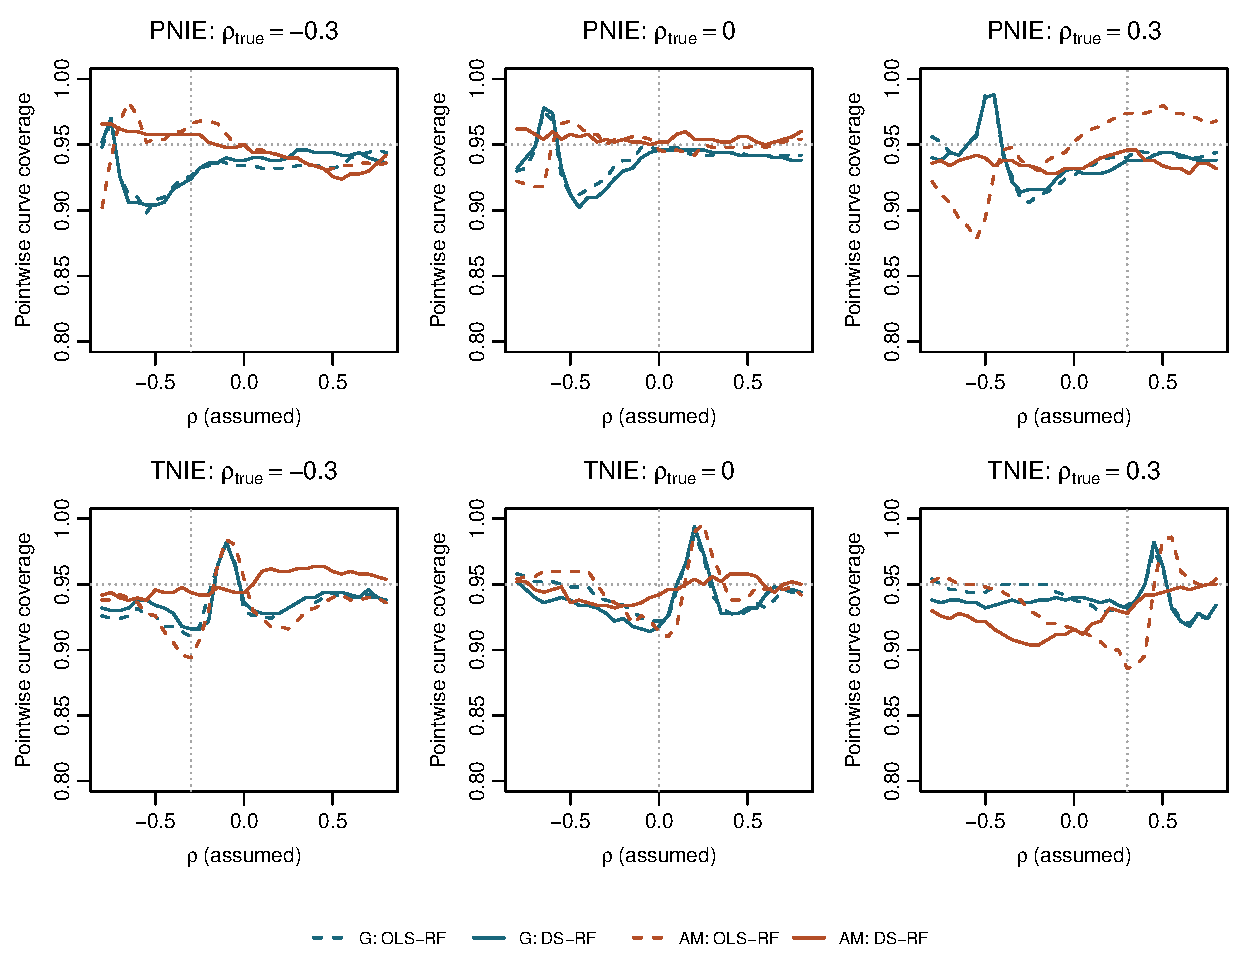
\includegraphics[width=0.98\textwidth]{figures/confounding_simulation_curve_coverage.pdf}
\caption{Pointwise coverage of the population sensitivity functional across the full assumed-correlation grid, conditional on numerical success. Each configuration starts with 500 attempts. G denotes Gaussian innovations and AM asymmetric-mixture innovations. The horizontal line is 0.95 and the vertical line is the generating correlation. At other correlations, coverage targets the corresponding sensitivity functional; at the generating correlation, that functional equals the generating causal effect. Complete Monte Carlo standard errors and report-and-cover fractions are retained in the project repository.}
\label{fig:curve-coverage}
\end{figure}

\begin{figure}[p]
\centering
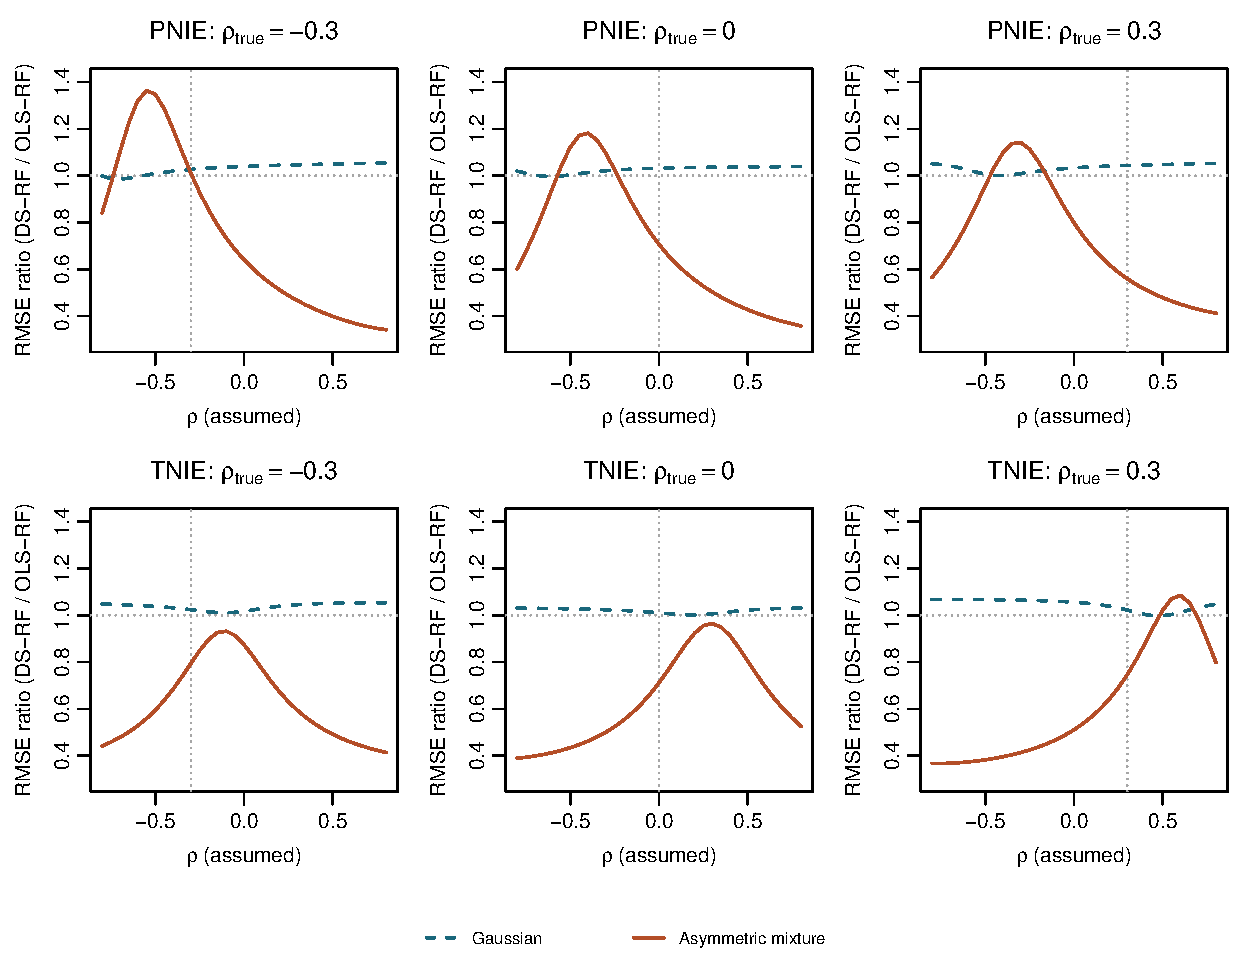
\includegraphics[width=0.98\textwidth]{figures/confounding_simulation_curve_ratios.pdf}
\caption{Paired DS-RF/OLS-RF RMSE ratios for the population PNIE/TNIE sensitivity curves. Ratios below one favor DS-RF in RMSE. The same successful data sets are used in the numerator and denominator, and all assumed correlations and generating configurations are retained. Pointwise coverage and numerical success provide the complementary calibration and reliability measures.}
\label{fig:curve-ratios}
\end{figure}

\begin{table}[htbp]\centering\small\setlength{\tabcolsep}{4pt}
\caption{Zero-boundary inference in the confounding simulation. The same retained data sets are used; these are not additional independent replications. Coverage and length refer to the Fisher-transform interval for $\rho_t^\dagger$.}
\label{tab:curve-thresholds}
\begin{tabular}{lrllrrrr}\toprule
Error & $\rho_{\rm true}$ & Effect & Method & Bias & RMSE & Coverage (MCSE) & Length\\\midrule
AM & -0.3 & PNIE & OLS-RF & 0.003 & 0.068 & 0.958 (0.009) & 0.276\\
AM & -0.3 & PNIE & DS-RF & 0.004 & 0.068 & 0.960 (0.009) & 0.275\\
AM & -0.3 & TNIE & OLS-RF & 0.001 & 0.078 & 0.940 (0.011) & 0.311\\
AM & -0.3 & TNIE & DS-RF & 0.002 & 0.077 & 0.944 (0.010) & 0.311\\
AM & 0.0 & PNIE & OLS-RF & 0.006 & 0.072 & 0.958 (0.009) & 0.290\\
AM & 0.0 & PNIE & DS-RF & 0.006 & 0.072 & 0.960 (0.009) & 0.290\\
AM & 0.0 & TNIE & OLS-RF & 0.008 & 0.081 & 0.946 (0.010) & 0.311\\
AM & 0.0 & TNIE & DS-RF & 0.007 & 0.081 & 0.944 (0.010) & 0.312\\
AM & 0.3 & PNIE & OLS-RF & -0.002 & 0.079 & 0.950 (0.010) & 0.306\\
AM & 0.3 & PNIE & DS-RF & -0.002 & 0.079 & 0.950 (0.010) & 0.305\\
AM & 0.3 & TNIE & OLS-RF & -0.003 & 0.080 & 0.936 (0.011) & 0.301\\
AM & 0.3 & TNIE & DS-RF & -0.004 & 0.079 & 0.936 (0.011) & 0.301\\
\midrule
G & -0.3 & PNIE & OLS-RF & 0.002 & 0.058 & 0.950 (0.010) & 0.215\\
G & -0.3 & PNIE & DS-RF & 0.002 & 0.058 & 0.948 (0.010) & 0.215\\
G & -0.3 & TNIE & OLS-RF & 0.002 & 0.080 & 0.954 (0.009) & 0.311\\
G & -0.3 & TNIE & DS-RF & 0.002 & 0.080 & 0.952 (0.010) & 0.311\\
G & 0.0 & PNIE & OLS-RF & 0.006 & 0.063 & 0.946 (0.010) & 0.243\\
G & 0.0 & PNIE & DS-RF & 0.006 & 0.063 & 0.946 (0.010) & 0.243\\
G & 0.0 & TNIE & OLS-RF & 0.005 & 0.081 & 0.944 (0.010) & 0.307\\
G & 0.0 & TNIE & DS-RF & 0.005 & 0.081 & 0.948 (0.010) & 0.307\\
G & 0.3 & PNIE & OLS-RF & 0.008 & 0.069 & 0.954 (0.009) & 0.274\\
G & 0.3 & PNIE & DS-RF & 0.008 & 0.069 & 0.954 (0.009) & 0.274\\
G & 0.3 & TNIE & OLS-RF & -0.000 & 0.069 & 0.946 (0.010) & 0.274\\
G & 0.3 & TNIE & DS-RF & -0.000 & 0.069 & 0.944 (0.010) & 0.274\\
\bottomrule\end{tabular}
\par\smallskip\begin{minipage}{0.98\textwidth}\footnotesize G: Gaussian; AM: asymmetric mixture. Each cell starts with 500 attempts. Success denominators and failure records are the same as for Table~\ref{tab:confounding-simulation}. A zero boundary of the point-estimate curve is not an interval-zero boundary.\end{minipage}
\end{table}


\clearpage
